\documentclass[tikz]{standalone}
\usetikzlibrary{shapes.geometric, arrows.meta, positioning}
\begin{document}
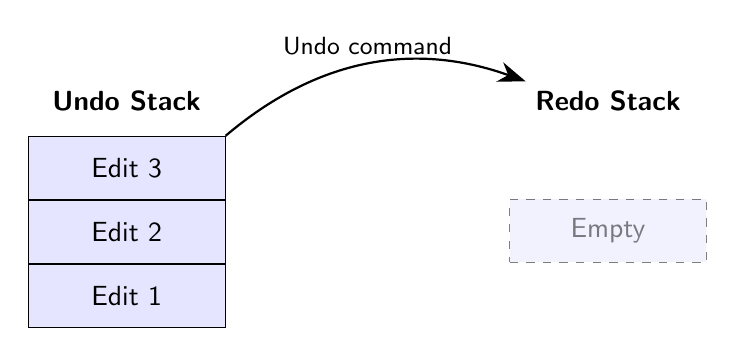
\begin{tikzpicture}[
    stack/.style={rectangle, draw, minimum width=2.5cm, minimum height=0.8cm, fill=blue!10, font=\sffamily},
    label/.style={font=\sffamily\bfseries}
]
    % Undo Stack
    \node[label] (undo_label) {Undo Stack};
    \node[stack, below=0.2cm of undo_label] (u3) {Edit 3};
    \node[stack, below=0cm of u3] (u2) {Edit 2};
    \node[stack, below=0cm of u2] (u1) {Edit 1};

    % Redo Stack
    \node[label, right=4cm of undo_label] (redo_label) {Redo Stack};
    \node[stack, below=1cm of redo_label, dashed, opacity=0.5] (r1) {Empty};

    % Arrow
    \draw[-{Stealth[scale=1.5]}, thick, bend left] (u3.north east) to node[above, font=\sffamily\small] {Undo command} (redo_label.north west);

\end{tikzpicture}
\end{document}